\documentclass[14pt,a4paper]{article}
\usepackage{mathtools}
\usepackage{amsmath}
\usepackage{amsthm}
\setcounter{MaxMatrixCols}{20}
\usepackage{mathrsfs}
\usepackage{setspace}
\usepackage{amsfonts}
\usepackage{geometry}
\geometry{a4paper, total = {210mm,297mm},left=25mm, right=20mm,top=25mm,bottom=25mm}
\usepackage{xcolor}
\usepackage{mcode}
\usepackage{listings}
\lstset{basicstyle = \fontsize{11}{12} \selectfont\ttfamily}
\usepackage{graphicx}


%Begin document - Numerical Analysis - Homework 5

\begin{document}
\label{cover}
\begin{center}
	\vspace*{3cm}
	\large{\textbf{MATH/CS 5466 NUMERICAL ANALYSIS \\ Homework 5}}
	\vfill
	\textbf{Luan Cong Doan} \\ luandoan@vt.edu
	%\vfill
%	Department of Mechanical Engineering \\ Virginia Polytechnic Institute and State University
	\vfill
	April 18, 2016
\end{center}
\pagebreak

\label{Answer Sheet - Numerical Homework 5}
\doublespacing

\label{Problem 1}
\large\textbf{Problem 1.} When tasked with computing a definite integral $\int_{a}^{b}f(x)\mathrm{d}x$, one is not forced to apply some quadrature rule directly to \textit{f}. Sometimes a bit of forethought can lead to a more effective approach.
\begin{enumerate}
	\label{1a}
	\item Does the standard error bound derived in class for the composite trapezoid rule give any insight about the performance of that method applied to the Fresnel integral
	$$ \int_{0}^{1}\dfrac{\sin(x)}{\sqrt{x}}\mathrm{d}x$$ 
	$f(x) = \dfrac{\sin(x)}{\sqrt{x}} \Rightarrow f'(x) = \dfrac{\cos(x)\sqrt{x} - \sin(x)\dfrac{1}{2\sqrt{x}}}{x} = \dfrac{2x\cos(x) - \sin(x)}{2x^{3/2}} $\\
	$ \hspace*{3.1cm} f''(x) = \dfrac{(2\cos(x) - 2x\sin(x) - \cos(x))2x^{3/2} - (2x\cos(x) - \sin(x))3x^{1/2}}{4x^3}$\\
	$ \hspace*{4.2cm} = \dfrac{2x^{3/2}\cos(x) - 4x^{5/2}\sin(x) - 6x^{3/2}\cos(x) + 3x^{1/2}\sin(x)}{4x^3}$\\
	$ \hspace*{4.2cm} = \dfrac{3x^{1/2}\sin(x) - 4x^{3/2}\cos(x) - 4x^{5/2}\sin(x)}{4x^3}$\\
	$ \hspace*{4.2cm} = \dfrac{3\sin(x) - 4x\cos(x) - 4x^2\sin(x)}{4x^{5/2}}$\\
		$f'''(x) =   \dfrac{\left[- \cos(x) - 4xsin(x) - 4x^2\cos(x)\right]4x^{5/2} - \left[3\sin(x) - 4x\cos(x) - 4x^2\sin(x)\right]10x^{3/2}}{16x^5}$
	We have: $f'''(x) < 0$ for all $x \in [0,1]$ $\Rightarrow f''(x)$ decreasing over $[0,1]$\\ 
	Error based on trapezoid rule:\\
	$E = -\dfrac{b-a}{12}h^2.f''(\eta) = -\dfrac{1}{12}h^2. \dfrac{3\sin(\eta) - 4\eta\cos(\eta) - 4\eta^2\sin(\eta)}{4\eta^{5/2}}$ \hspace{0.5cm} for some $\eta \in [0,1]$\\
	$ \hspace*{3.8cm} =-\dfrac{1}{12}h^2.\left( \dfrac{3\sin(\eta)}{4\eta^{5/2}} - \dfrac{\cos(\eta)}{\eta^{3/2}} - \dfrac{\sin(\eta)}{\eta^{1/2}}\right)$\\
	We easily see that: $\lim\limits_{\eta \rightarrow 0}E = \infty$\\
	$\Rightarrow$ NO insight for error bound for Fresnel integral based on composite trapezoid rule. 
	
	\label{1b}
	\item One can compute this Fresnel integral by expanding $\sin(x)$ in a Taylor series about $x=0$ to obtain
	$$\int_{0}^{\varepsilon}\left(\dfrac{x - \frac{1}{3!}x^3 + ...}{\sqrt{x}}\right)\mathrm{d}x + \int_{\varepsilon}^{1}\dfrac{\sin(x)}{\sqrt{x}}\mathrm{d}x$$
	To approximate this quantity, truncate the Taylor series after $m$ terms and compute the resulting approximation to the first integral exactly; approximate the second integral using the composite trapezoid rule. Estimate the accuracy of this procedure as a function of $m,\epsilon$, and the number of subintervals used in the composite trapezoid rule for the second integral.\\
	Expansion of function $\sin(x)$ to $m$ terms by using Taylor series:\\
	\hspace*{2cm}$\sin(x) = x - \dfrac{x^3}{3!} + \dfrac{x^5}{5!} - \dfrac{x^7}{7!} + ... + (-1)^{m}\dfrac{x^{2m+1}}{(2m+1)!} $ \hspace{1cm} for $m = 0,1,2, ...$\\
	We have the first integral with $m$ terms:
	\begin{align*} \int_{0}^{\varepsilon}\left(\dfrac{x - \frac{1}{3!}x^3 + ...}{\sqrt{x}}\right)\mathrm{d}x &= \int_{0}^{\varepsilon} \left(x^{1/2} - \dfrac{1}{3!}x^{5/2} +  ... + (-1)^{m}\dfrac{1}{(2m+1)!}x^{(4m+1)/2} \right) \mathrm{d}x \\
	&= \left.\left( \dfrac{2}{3}x^{3/2} - \dfrac{2}{7}\dfrac{1}{3!}x^{7/2} +  ... + (-1)^m\dfrac{2}{4m+1}\dfrac{1}{(2m+1)!}x^{(4m+1)/2} \right)\right|_0^{\varepsilon}\\
	&= \dfrac{2}{3}\varepsilon^{3/2} - \dfrac{2}{7}\dfrac{1}{3!}\varepsilon^{7/2} +  ... + (-1)^m\dfrac{2}{4m+1}\dfrac{1}{(2m+1)!}\varepsilon^{(4m+1)/2}
	\end{align*}
	Second integral can be compute via composite trapezoid rule: $h = \dfrac{1-\varepsilon}{N}$ with $N$ is number of subinterval
	\begin{align*} \int_{\varepsilon}^{1}\dfrac{\sin(x)}{\sqrt{x}}\mathrm{d}x &= \dfrac{h}{2}\left[ f(x_0) + 2\sum_{j=1}^{N-1}f(x_j) + f(x_N)\right] -\dfrac{1-\varepsilon}{12}h^2.f''(\eta) \\
	&= \dfrac{1-\varepsilon}{2N}\left[ \dfrac{\sin(\varepsilon)}{\sqrt{\varepsilon}} + 2\sum_{j=1}^{N-1} \dfrac{\sin(\varepsilon + j\dfrac{1-\varepsilon}{N})}{\sqrt{\varepsilon+j\dfrac{1-\varepsilon}{N}}} + \dfrac{\sin(1)}{\sqrt{1}}  \right] - \dfrac{(1-\varepsilon)^3}{12N^2}.f''(\eta)
	\end{align*}
	Error: $E_2 = - \dfrac{(1-\varepsilon)^3}{12N^2}.f''(\eta)= - \dfrac{(1-\varepsilon)^3}{12N^2}\left[ \dfrac{3\sin(\eta)}{4\eta^{5/2}} - \dfrac{\cos(\eta)}{\eta^{3/2}} - \dfrac{\sin(\eta)}{\eta^{1/2}}\right]$ with $\eta \in [\varepsilon,1]$\\
	Base on above result, we have $f''(\eta)$ decreasing over $[\varepsilon,1] \Rightarrow \min(f''(\eta)) = f''(\varepsilon)$
	$$\Rightarrow E_2 = - \dfrac{(1-\varepsilon)^3}{12N^2}.f''(\eta) \leq - \dfrac{(1-\varepsilon)^3}{12N^2}\left[ \dfrac{3\sin(\varepsilon)}{4\varepsilon^{5/2}} - \dfrac{\cos(\varepsilon)}{\varepsilon^{3/2}} - \dfrac{\sin(\varepsilon)}{\varepsilon^{1/2}}\right]$$
	So:
	$$ \int_{\varepsilon}^{1}\dfrac{\sin(x)}{\sqrt{x}}\mathrm{d}x \leq 	\dfrac{h}{2}\left[ \dfrac{\sin(\varepsilon)}{\sqrt{\varepsilon}} + 2\sum_{j=1}^{N-1} \dfrac{\sin(\varepsilon + jh)}{\sqrt{\varepsilon+jh}} + \sin(1)  \right] - \dfrac{(1-\varepsilon)^3}{12N^2}\left[ \dfrac{3\sin(\varepsilon)}{4\varepsilon^{5/2}} - \dfrac{\cos(\varepsilon)}{\varepsilon^{3/2}} - \dfrac{\sin(\varepsilon)}{\varepsilon^{1/2}}\right]$$
	
	
	\label{1c}
	\item Construct a function $g(x)$ such that the integral in part (a) can be effectively computed:	
	$$\int_{0}^{1}\left( \dfrac{\sin(x)}{\sqrt{x}} - g(x)\right)\mathrm{d}x + \int_{0}^{1}g(x)\mathrm{d}x$$
	where the first integral can be computed with the composite trapezoid rule and the second integral can be computed exactly without need for numerical quadrature. \\
	As result from above, we have the composite trapezoid approximation for $\int_{0}^{1}f(x)\mathrm{d}x$ is:
	\begin{align*} \int_{0}^{1}\dfrac{\sin(x)}{\sqrt{x}}\mathrm{d}x &= \dfrac{h}{2}\left[ \dfrac{\sin(0)}{\sqrt{0}} + 2\sum_{j=1}^{N-1} \dfrac{\sin(0 + jh)}{\sqrt{0+jh}} + \sin(1)  \right] - \dfrac{1}{12N^2}\left[ \dfrac{3\sin(\eta)}{4\eta^{5/2}} - \dfrac{\cos(\eta)}{\eta^{3/2}} - \dfrac{\sin(\eta)}{\eta^{1/2}}\right]\\
	&= \dfrac{h}{2}\left[2\sum_{j=1}^{N-1} \dfrac{\sin(jh)}{\sqrt{jh}} + \sin(1)  \right] - \dfrac{1}{12N^2}\left[ \dfrac{3\sin(\eta)}{4\eta^{5/2}} - \dfrac{\cos(\eta)}{\eta^{3/2}} - \dfrac{\sin(\eta)}{\eta^{1/2}}\right] \hspace{1cm} \eta \in [0,1]
	\end{align*}
	We can not get the exact result of approximation because terms in error part are not bounded. So, utilizing Taylor expansion for $\sin(x)$ and $\cos(x)$ we have:
	$$ \sin(x) = x - \dfrac{x^3}{3!} + \dfrac{x^5}{5!} + ... = \sum_{n=0}^{\infty} \dfrac{(-1)^n}{(2n+1)!}x^{2n+1}$$
	$$\cos(x) = x - \dfrac{x^2}{2!} + \dfrac{x^4}{4!} + ... = \sum_{n=0}^{\infty} \dfrac{(-1)^n}{(2n)!}x^{2n}$$
	\begin{align*} Error &= - \dfrac{1}{12N^2}\left[ \dfrac{3\sin(\eta)}{4\eta^{5/2}} - \dfrac{\cos(\eta)}{\eta^{3/2}} - \dfrac{\sin(\eta)}{\eta^{1/2}}\right]\\ 
	&= - \dfrac{1}{12N^2}\left[\dfrac{1}{\eta^{5/2}}\sum_{n=0}^{\infty} \dfrac{(-1)^n}{(2n+1)!}\eta^{2n+1} - \dfrac{1}{\eta^{3/2}}\sum_{n=0}^{\infty} \dfrac{(-1)^n}{(2n)!}\eta^{2n} - \dfrac{1}{\eta^{1/2}} \sum_{n=0}^{\infty} \dfrac{(-1)^n}{(2n+1)!}\eta^{2n+1}\right]\\
	&= - \dfrac{1}{12N^2}\left[\dfrac{1}{\eta^{3/2}} + \sum_{n=1}^{\infty} \dfrac{(-1)^n}{(2n+1)!}\eta^{2n-3/2} - \dfrac{1}{\eta^{1/2}} - \sum_{n=1}^{\infty} \dfrac{(-1)^n}{(2n)!}\eta^{2n-3/2} - \sum_{n=0}^{\infty} \dfrac{(-1)^n}{(2n+1)!}\eta^{2n+1/2}\right]
	\end{align*}
	In order to get the right value of error, we have to neglect 2 terms: $\dfrac{1}{\eta^{3/2}}$, and $\dfrac{1}{\eta^{1/2}}$ in error function. So we have:
	$$\int_{0}^{1}g(x)\mathrm{d}x = - \dfrac{1}{12N^2}\left[\dfrac{1}{\eta^{3/2}} - \dfrac{1}{\eta^{1/2}}\right] = - \dfrac{1}{12N^2}\left[\eta^{-3/2} - \eta^{-1/2}\right] \Leftrightarrow $$
	The easiest solution could be: $g(x) = - \dfrac{1}{12N^2}\left[\eta^{-3/2} - \eta^{-1/2}\right]$ for some $\eta \in [0.1]$\\
	
\end{enumerate}
\pagebreak

\label{Problem 2}
\large\textbf{Problem 2.} The gamma function is defined as
$$\Gamma(z) = \int_{0}^{\infty}x^{z-1}e^{-x}\mathrm{d}x$$
 
\begin{enumerate}
	\label{2a} 
	\item Use the composite Simpson's rule to evaluate $\Gamma(5), \Gamma(10)$, and $\Gamma(0.5)$ to five digits of accuracy. You may use \texttt{MATLAB}'s built-in \texttt{gamma} function to verify your answer. Please report the number of integrand evaluations required. In particular, design a way to reliably compute $\Gamma(0.5)$ using fewer than 1000 function evaluation. (Consider further partitioning the domain into subdomains).
	\begin{lstlisting}
	G5 = gamma(5);
	G10 = gamma(10);
	Gd5 = gamma(0.5);
	
	Result: 	>> G5	G5 = 24
				>> G10	G10 = 362880
				>> Gd5	Gd5 = 1.772524
	
	\end{lstlisting}
	
	
	The orthogonal polynomial on $[0, \infty)$ with weight function $w(x) = e^{-x}$ are called Gauss-Laguerre polynomials. These polynomials can be constructed from the recurrence\\
	$L_0(x) = 1, \hspace{0.2cm} L_1(x) = x-\alpha_0 = x-1, \hspace{0.2cm} L_{k+1}(x) = (x-\alpha_k)L_k(x)-\beta_kL_{k-1}(x)$, \hspace{0.2cm} $k = 1,2, ...$\\
	where $\alpha_k = 2k+1$ for $k = 0,1, ...$ \hspace{0.2cm} $\beta_0 = 1$, and $\beta_k = k^2$ for $k = 1,2, ...$\\
		
	\label{2b}	
	\item Use your answer from Question 3 of Problem Set 4 to design a \texttt{MATLAB} function:\\ \hspace*{5cm} \texttt{[x,w] = gauss\_lag(n)}\\
	that computes the nodes $x$ and the weight $w$ for $n+1$ point Gauss-Laguerre quadrature from the corresponding Jacobi matrix \textbf{J}. Recall that the weights are given by $w_j = \beta_0(\textbf{v}_j)_1^2$ \\
	where $(\textbf{v}_j)_1^2$ is the square of the first entry of the eigenvector $\textbf{v}_j$ of \textbf{J} corresponding to the eigenvalue $x_j$. (Here $\textbf{v}_j$ should be normalized so that $\|\textbf{v}_j\|_2 = 1$, which is automatically imposed upon the eigenvectors returned by \texttt{MATLAB's eig} command).\\
	$ L_{k+1}(x) = (x-\alpha_k)L_k(x)-\beta_kL_{k-1}(x) = xL_k(x) - \alpha_kL_k(x) - \beta_kL_{k-1}(x)$\\
	\hspace*{6.8cm} $= xL_k(x) - (2k+1)L_k(x) - k^2L_{k-1}(x)$\\
	and $L_0 = 1, L_1(x) = x - \alpha_0 = x-1$\\
	As result from Question 3 - Problem set 4 we have the corresponding Jacobi matrix \textbf{J} is defined by:\\
	\hspace*{1cm} $ \textbf{J} = \begin{bmatrix} \alpha_0 & \sqrt{\beta_1} & 0 & ... & 0 \\ \sqrt{\beta_1} & \alpha_1 & \sqrt{\beta_2} & ... & 0 \\ 0 & \sqrt{\beta_2} & \ddots & \ddots \\ ...&...&...&...&...\\ 0 & 0 & \ddots & \alpha_{n-1} & \sqrt{\beta_n} \\ 0 & 0 & ... & \sqrt{\beta_n} & \alpha_n \end{bmatrix} = \begin{bmatrix} 1 & 1 & 0 & ... & 0 \\ 1 & 3 & 2 & ... & 0 \\  & 2 & \ddots & \ddots \\...&...&...&...&...\\ 0 & 0 & \ddots & 2n-1 & n \\ 0 & 0 & ... & n & 2n+1 \end{bmatrix}$
	\begin{lstlisting}
	function [x,w] = gauss_lag(n)
	J = zeros(n+1);	x = zeros(1,n+1);
	for i = 1:n+1
		for j = 1:n+1
			if (i-j==0) 		J(i,j) = 2*i-1;
			elseif (j-i==1)		J(i,j) = i;
			elseif (i-j==1)		J(i,j) = j;
			end
		end
	end
	[V,D] = eig(J);
	for i = 1:size(D,1)
		for j = 1:size(D,2)
			if (i-j==0)		x(1,i) = D(i,j);	end
		end
	end
		w = V(1,:).^2;
	\end{lstlisting}
	
			
	\label{2c}
	\item Produce a \textit{single plot} comparing the nodes of all $n+1$ point Gauss-Laguerre rules for $n=0,...,25$. For example, you can plot each set of nodes with\\
	\hspace*{5cm} \texttt{plot(x, n*ones(n+1,1), '.','markersize',24)}\\
	which displays the nodes horizontally at vertical level $n$. (Notice how the largest node, $x_n$, grows as $n$ increases, as the rule integrates over the unbounded interval $[0, \infty)$.)
	\begin{lstlisting}
	N = 1:1:25;
	figure;
	for i = 1:length(N)
		[x,~,~] = gauss_lag(i);
		plot(x, i*ones(i+1,1), '.','markersize',24); hold on; grid on;
	end
	xlabel('x'); ylabel('N'); title('Root estimation');
	print('hw5_2c','-dpng');
	\end{lstlisting}
	\begin{figure}[htp]
		\centering
		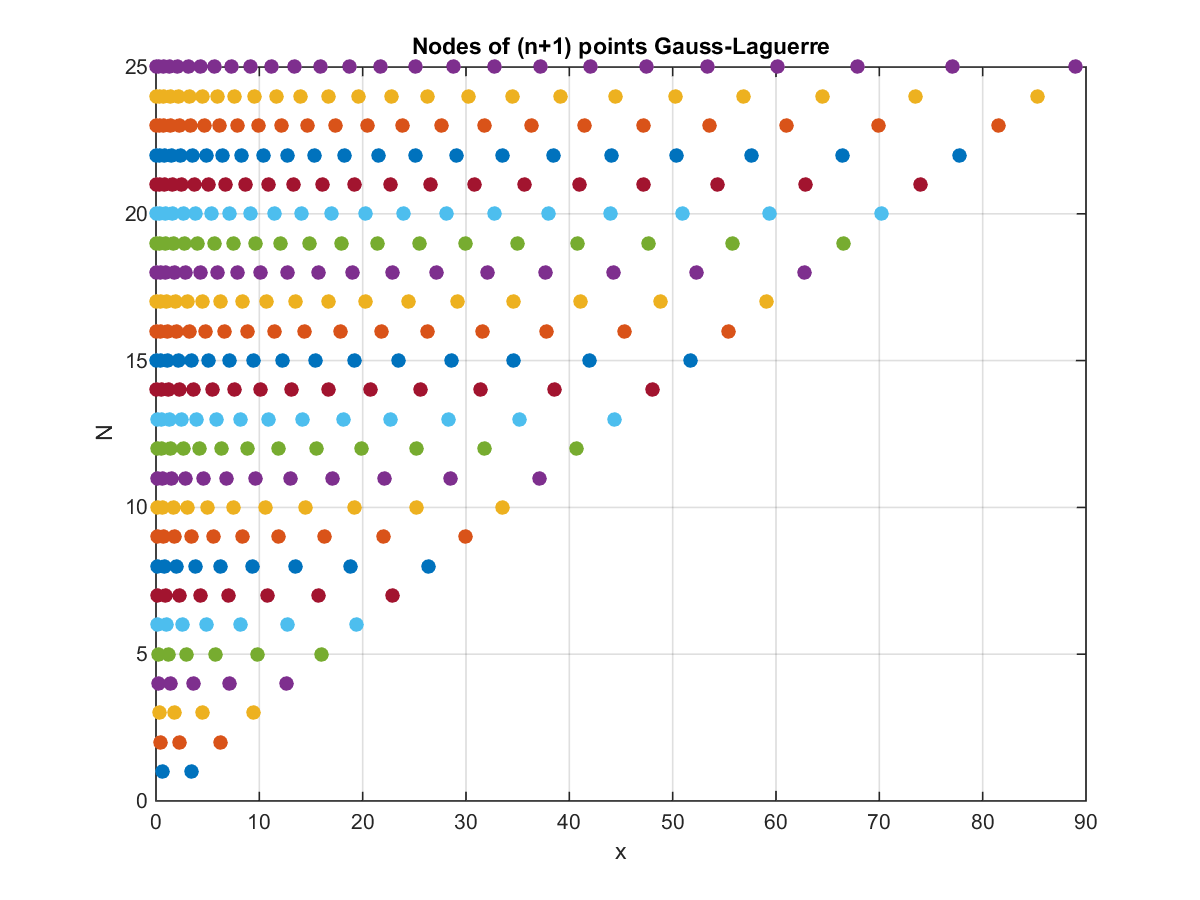
\includegraphics[scale=0.6]{hw5_2c.png}
		\caption{Nodes of ($n+1$) points Gauss-Laguerre}
	\end{figure}
	
	
	\label{2d}
	\item Compute $\Gamma(5), \Gamma(10)$, and $\Gamma(0.5)$ using this $n+1$ point Gauss-Laguerre rule for $n=5$. (Each of these integrals will only require six $ f(x)$ evaluations.)
	$$\Gamma(z) = \int_{0}^{\infty}x^{z-1}e^{-x}\mathrm{d}x = \sum_{0}^{\infty}w_if(x_i)$$
	
	\label{2e} 
	\item How does the accuracy of Gauss-Laguerre quadrature compare to that obtained by the composite Simpson's rule? Give pros and cons of each method for this problem.
	
	 
\end{enumerate}

\label{Problem 3}
\large\textbf{Problem 3.} How might the implementer of a mathematical function library (or even hardware designer) implement a function like \texttt{sqrt} using only basic operations (addition, subtraction, multiplication, division)? Various clever approaches exist. This question (from problems in Gautschi's book) considers several options using Newton's method.
\begin{enumerate}
	\label{3a}
	\item Given some fixed $A > 0$, one can compute $x_* = \sqrt{A}$ via the root-finding problem: $x^2 - A = 0$
	Explain why Newton's method applied to the first equation converges for any initial value $x_0 > 0$. Be as rigorous as possible. \\
	\hspace*{2cm}	$f_1(x) = x^2 - A \rightarrow f_1'(x) = 2x$\\
	\hspace*{5.3cm}	$f_1''(x) = 2 > 0 \rightarrow f_1(x)$ is convex on $\mathbb{R}_+$ \\
	and increase monotonically from $-A$ to $\infty$.\\
	Therefore, if $x_0 > \alpha$ ($\alpha = \sqrt{A}$), then $x_n$ converges monotonically decreasing to $\alpha$. \\
	If $0 < x_0 < \alpha$, then $x_1 > \alpha$, and the same conclusion holds for $n \geq 1$.
	
	
	\label{3b}
	\item Alternatively, one might compute $x_* = \sqrt{A}$ via the root-finding problem: $\dfrac{A}{x^2} -1 = 0$\\
	Show that the initial set of positive initial guesses $x_0 > 0$ can be partitioned into three sets:\\
	\hspace*{2cm} $x \in (0,\alpha) \Rightarrow x_k \rightarrow \sqrt{A}$ and all $x_k > 0$\\
	\hspace*{2cm} $x \in (\alpha, \beta) \Rightarrow x_k \rightarrow \pm \sqrt{A}$, $x_k$ do not all have the same sign;\\
	\hspace*{2cm} $x \in (\beta, \infty) \Rightarrow x_k $ diverges\\
	(You should specify formulas for $\alpha$ and $\beta$ as a function of A)\\
	\hspace*{2cm}	$f_2(x) = \dfrac{A}{x^2} - 1 \rightarrow f_2'(x) = -\dfrac{2A}{x^3}$\\
	\hspace*{5.3cm}	$f_2''(x) = \dfrac{6A}{x^4} > 0 \rightarrow f_2(x)$ is convex on $\mathbb{R}_+$ \\
	and decrease monotonically from $\infty$ to $-1$. \\
	If $0 < x_0 < \alpha$ ($\alpha = \sqrt{A}$) then $x_n$ converges monotonically increasing to $\alpha$.\\
	If $x_0 > \alpha$, we must make sure that $x_1 > 0$, which following Newton-method means that: \\
	$ x_1 = x_0 - \dfrac{f(x_0)}{f'(x_0)} > 0 \Leftrightarrow x_1 = x_0 - \dfrac{\frac{A}{x_0^2} -1}{-2\frac{A}{x_0^3}} > 0 \Leftrightarrow x_0 + x_0\dfrac{A - x_0^2}{2A} > 0 $\\
	\hspace*{8.3cm} $\Leftrightarrow 3Ax_0 - x_0^3 > 0 $\\
	\hspace*{8.3cm} $\Leftrightarrow 3A - x_0^2 > 0 $\\
	\hspace*{8.3cm} $\Leftrightarrow x_0 < \sqrt{3A} =: \beta$\\
	
	\label{3c}
	\item Repeat part (a) and (b) for the analogous approaches to the cube root:\\
	\hspace*{3cm} $x^3 - A = 0; \hspace{2cm} \dfrac{A}{x^3} - 1 = 0$\\
	In generalizing part (b), simplify identify the interval $(0,\alpha)$ (with $\alpha = \sqrt[3]{A}$) on which the iterates are all positive and coverage to $\sqrt{A}$\\
	\hspace*{2cm}	$f_3(x) = x^3 - A \rightarrow f_3'(x) = 3x^2$\\
	\hspace*{5.3cm}	$f_3''(x) = 6x > 0 $ because $ x > 0$\\
	$\rightarrow f_3(x)$ is convex on $\mathbb{R}_+$ and increasing monotonically from $-A$ to $\infty$.\\
	Then, if $x_0 > \alpha$, then $x_n$ converges monotonically decreasing to $\alpha$. \\
	If $0 < x_0 < \alpha$, then $x_1 > \alpha$, and the same conclusion holds for $n \geq 1$.\\
		
	\hspace*{2cm}	$f_4(x) = \dfrac{A}{x^3} - 1 \rightarrow f_4'(x) = -\dfrac{3A}{x^4}$\\
	\hspace*{5.3cm}	$f_4''(x) = \dfrac{12A}{x^5} > 0$ because $x > 0$\\
	$\rightarrow f_4(x)$ is convex on $\mathbb{R}_+$ and decrease monotonically from $\infty$ to $-1$\\
	If $0 < x_0 < \alpha$ then $x_n$ converges monotonically increasing to $\alpha$.\\
	If $x_0 > \alpha$, we must make sure that $x_1 > 0$, which following Newton-method means that: \\
	$ x_1 = x_0 - \dfrac{f(x_0)}{f'(x_0)} > 0 \Leftrightarrow x_1 = x_0 - \dfrac{\frac{A}{x_0^3} -1}{-3\frac{A}{x_0^4}} > 0 \Leftrightarrow x_0 + x_0\dfrac{A - x_0^4}{3A} > 0 $\\
	\hspace*{8.3cm} $\Leftrightarrow 4Ax_0 - x_0^4 > 0 $\\
	\hspace*{8.3cm} $\Leftrightarrow 4A - x_0^3 > 0 $\\
	\hspace*{8.3cm} $\Leftrightarrow x_0 < \sqrt[3]{4A} =: \beta$\\
	
	
	\label{3d}
	\item One can also compute to compute $x_* = \sqrt{A}$ via the fixed point iteration:\\
	\hspace*{5cm} $x_{k+1} =  \dfrac{x_k(x_k^2 + 3a)}{3x_k^2 + a}$\\
	(i) Show that \textit{if the sequence converges to} $\sqrt{A}$, it converges \textit{cubucally}\\
	(ii) Determine the \textit{asymptotic error constant} \\
	(iii) Discuss (using graphical or numerical support) the convergence of this method $x_0 > 0$.\\
	Set $\varphi(x) = \dfrac{x_k(x_k^2 + 3a)}{3x_k^2 + a}, \hspace{1cm} \alpha = \sqrt{a}$\\
	Clearly see that: $\Rightarrow \varphi(\alpha) = \dfrac{\alpha(\alpha^2 + 3a)}{3\alpha^2 + a} = \dfrac{\alpha(a+3a)}{3a +a} =\alpha$\\
	We have: $(3x^2 + a)\varphi(x) = x^3 + 3ax$\\
	Differentiating above equation: $6x\varphi(x) + (3x^2 + a)\varphi'(x) = 3x^2 + 3a$ \\
	At $x = \alpha$:  $6\alpha\varphi(\alpha) + (3\alpha^2 + a)\varphi'(\alpha) = 3\alpha^2 + 3a \Leftrightarrow 6\alpha\varphi(\alpha) + 6a\varphi'(\alpha) = 6a $ \\
	\hspace*{8.6cm} $ \Leftrightarrow 6\alpha\alpha + 4a\varphi'(\alpha) = 6a $ \\
	\hspace*{8.6cm} $ \Leftrightarrow \varphi'(\alpha) = 0 $ \\
	Second order differentiation equation: $6\varphi(x) + 6x\varphi'(x) + 6x\varphi'(x) + (3x^2 + a)\varphi''(x) = 6x$ \\
	\hspace*{6.3cm} $\Leftrightarrow 6\varphi(x) + 12x\varphi'(x) + (3x^2 + a)\varphi''(x) = 6x$ \\
	At $x = \alpha$: $6\varphi(\alpha) + 12\alpha\varphi'(\alpha) + (3\alpha^2 + a)\varphi''(\alpha) = 6\alpha \Leftrightarrow 4a\varphi''(\alpha) = 0 \Leftrightarrow \varphi''(\alpha) = 0 $ \\
	Third order differentiation equation:\\
	\hspace*{2.6cm} $6\varphi'(x) + 12\varphi'(x) + 12x\varphi''(x) + 6x\varphi''(x) + (3x^2 + a)\varphi'''(x) = 6$ \\
	\hspace*{2cm} $\Leftrightarrow 18\varphi'(x) + 18x\varphi''(x) + (3x^2 + a)\varphi'''(x) = 6$ \\
	At $x = \alpha$: $18\varphi'(\alpha) + 18\alpha\varphi''(\alpha) + (3\alpha^2 + a)\varphi'''(\alpha) = 6 \Leftrightarrow 4a\varphi'''(\alpha) = 6 \Leftrightarrow \varphi'''(\alpha) = \dfrac{6}{4a} \neq 0 $ \\
	$\Rightarrow$ the iteration converges at order $p = 3$ or \textit{cubically}\\
	The \textit{asymptotic error constant} is determined by:\\
	\hspace*{4cm} $ c= \dfrac{1}{3!}\varphi'''(\alpha) = \dfrac{1}{6}\dfrac{6}{4a} = \dfrac{1}{4a}$\\
	Applied Taylor expansion for $\varphi(x_0)$ at $\alpha$ we have:\\
	$\varphi(x_0) = \varphi(\alpha) + \varphi'(\alpha)(x_0 -\alpha) + \dfrac{\varphi''(\alpha)}{2!}(x_0-\alpha)^2 + \dfrac{\varphi'''(\xi)}{3!}(x_0-\alpha)^3$ \hspace{0.5cm} for some $\xi \in [x_0,\alpha]$\\
	$ \Leftrightarrow x_1 = \alpha - \dfrac{\varphi'''(\xi)}{6}(x_0-\alpha)^3$ \hspace{2cm} because $\alpha = \varphi(\alpha)$ and $\varphi'(\alpha) = \varphi''(\alpha) = 0$\\
	\hspace*{0.5cm}	$ \Leftrightarrow e_1 = - \dfrac{\varphi'''(\xi)}{6}e_0^3$\\
	In general, the convergence of this method is: $e_{k+1} = - \dfrac{\varphi'''(\xi)}{6}e_k^3$ \hspace{0.5cm} for some $\xi \in [x_k,\alpha]$\\
	
\end{enumerate}

\label{Problem 4}
\large\textbf{Problem 4.} Recall the derivation of Newton's method: A function $f \in C^2(\mathbb{R})$ was expanded in a Taylor series up to first order. Here we investigate the algorithm obtained by taking one more term in the Taylor series. Assume $f \in C^3(\mathbb{R})$.

\begin{enumerate}
	\label{4a}
	\item Derive an algorithm analogous to Newton's method but based on the first three terms of the Taylor series for $f(x_*)$ expanded at $f(x_k)$ rather than just the first two. This method should include evaluations of both $f'(x_k)$ and $f''(x_k)$\\ 
	Taylor expansion of $f(x_*)$ at $x_k \approx x_*$ for first three term:\\
	$f(x_*) = f(x_k) + f'(x_k)(x_* - x_k) + \dfrac{f''(x_k)}{2!}(x_* - x_k)^2 + \dfrac{f'''(\xi)}{3!}(x_*-x_k)^3$ for some $\xi \in [x_k,x_*]$ \\
	Neglect the third order term:\\
	\hspace*{2cm}	$ 0 = f(x_k) + f'(x_k)(x_{k+1}-x_k) + \dfrac{f''(x_k)}{2!}(x_{k+1} - x_k)^2$\\
	\hspace*{1.4cm} $ \Leftrightarrow f''(x_k)x_{k+1}^2 - 2f''(x_k)x_kx_{k+1} + 2f'(x_k)x_{k+1} + 2f(x_k) - 2f'(x_k)x_k = 0$\\
	\hspace*{1.4cm} $ \Leftrightarrow f''(x_k)x_{k+1}^2 - 2\left[f''(x_k)x_k - f'(x_k)\right]x_{k+1} + 2f(x_k) - 2f'(x_k)x_k = 0$\\
	\hspace*{3cm} $\Delta = 4 \left[(f''(x_k)x_k - f'(x_k)\right]^2 - 8f''(x_k)\left[f(x_k) - f'(x_k)x_k\right]$\\
	\hspace*{1cm} $\Rightarrow x_{k+1} = \dfrac{2\left[(f''(x_k)x_k - f'(x_k)\right] - \sqrt{\Delta}}{2f''(x_k)}$ \hspace{1cm} or \hspace{0.5cm} $x_{k+1} = \dfrac{2\left[(f''(x_k)x_k - f'(x_k)\right] + \sqrt{\Delta}}{2f''(x_k)}$\\
	
	\label{4b}	
	\item At each iteration, Newton's method approximates the root of $f$ by the root of the line tangent to $f$ at $x_k$. Your new algorithm should approximate $f$ by a parabola. Draw this parabola, together with the tangent line used by Newton's method, for the function $f(x) = \sin(x)e^x$ at the point $x_0 = 1.25$. (Please produce a careful \texttt{MATLAB} plot, not a hand-drawn sketch).
	\begin{lstlisting}
	x = -1:0.05:2;
	f = sin(x).*exp(x);
	fx = sin(1.25).*exp(1.25);
	f1x = cos(x).*exp(x) + sin(x).*exp(x);
	f1 = cos(1.25).*exp(1.25) + sin(1.25).*exp(1.25);
	f2x = 2*cos(x).*exp(x);
	f2 = 2*cos(1.25).*exp(1.25);
	N2 = f1*(x-1.25) + fx;
	N3 = f2*x.^2 -2*(f2*1.25-f1)*x + 2*(fx-f1*1.25);
	figure; plot(x,f,'k','linewidth',1); grid on; hold on;
	plot(x,N2,'r--'); plot(x,N3,'b.');
	xlabel('x'); ylabel('f(x) = sin(x).e^x');
	title('Newton method approximation of root at x_0 = 1.25');
	legend('fx','tangent line','parabola');
	print('hw5_4b','-dpng');
	\end{lstlisting}
	\begin{figure}[htp]
		\centering
		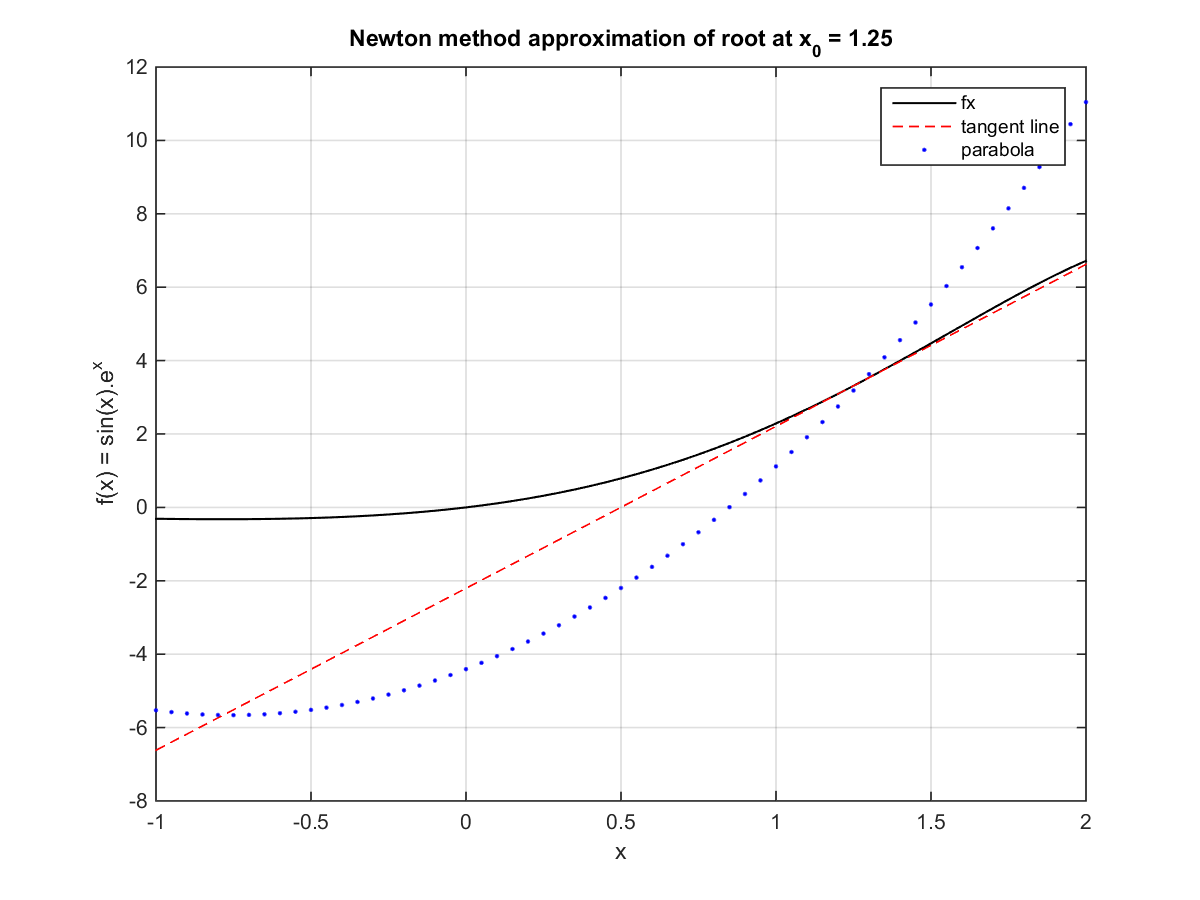
\includegraphics[scale=0.7]{hw5_4b.png}
		\caption{Newton's method approximation of root of $f(x) = \sin(x)e^x$}
	\end{figure}
		
	\label{4c}
	\item The parabola in question will often have two roots. Describe which of these roots should be selected at each iteration.\\
	The parabola equation have 2 roots: $x_{k1} < x_{k2}$ with values computed in part (a).\\
	The subinterval is defined by $[a,b]$, and current iteration point is $x_k: a\leq x_k \leq b$ \\
	$\Rightarrow$ the suitable root will be chosen by following steps:\\
	+ Check: $x_{k1}, x_{k2} \in [a,b]$, which is not meet this requirement should be neglected. \\
	+ If $a \leq x_{k1} < x_{k2} \leq x_k < b$, check sign of: $f(x_k)*f(x_{k1}),  f(x_k)*f(x_{k2})$\\
	\hspace*{2cm} $\bullet$ If $\begin{cases} f(x_k)*f(x_{k1}) < 0 \\ f(x_k)*f(x_{k2}) > 0 \end{cases} \Rightarrow $ new iteration point is $x_{k2}$\\
	\hspace*{2cm} $\bullet$ If $\begin{cases} f(x_k)*f(x_{k1}) > 0 \\ f(x_k)*f(x_{k2}) > 0 \end{cases} \Rightarrow $ new iteration point is $x_{k1}$\\
	+ If $a < x_k \leq x_{k1} < x_{k2} \leq b$, check sign of: $f(x_k)*f(x_{k1}),  f(x_k)*f(x_{k2})$\\
	\hspace*{2cm} $\bullet$ If $\begin{cases} f(x_k)*f(x_{k1}) > 0 \\ f(x_k)*f(x_{k2}) > 0 \end{cases} \Rightarrow $ new iteration point is $x_{k2}$\\
	\hspace*{2cm} $\bullet$ If $\begin{cases} f(x_k)*f(x_{k1}) > 0 \\ f(x_k)*f(x_{k2}) < 0 \end{cases} \Rightarrow $ new iteration point is $x_{k1}$\\
		
	\label{4d}
	\item Under what circumstances will this parabola have no roots?\\
	As result from part (a), parabola have no root when:
	\begin{align*} \Delta &= 4 \left[(f''(x_k)x_k - f'(x_k)\right]^2 - 8f''(x_k)\left[f(x_k) - f'(x_k)x_k\right] < 0\\
	&\Leftrightarrow 4(f''(x_k)x_k)^2 + 4(f'(x_k))^2 - 8f''(x_k)f(x_k) < 0 \\
	&\Leftrightarrow (f''(x_k)x_k)^2 + (f'(x_k))^2 - 2f''(x_k)f(x_k) < 0 \end{align*}

	
	\label{4e}
	\item Implement this algorithm in \texttt{MATLAB}, in a form similar to the code \texttt{newton.m} discussed in class
	\begin{lstlisting}
	 function xstar = newton2(f,fprime,f2prime, x0)
	 maxit = 60; 
	 fx = feval(f,x0); x=x0; k=0;       % initialize
	 fprintf(' %3d  %20.14f  %10.7e\n', k, x, fx);
	 while (abs(fx) > 1e-15) && (k < maxit)
	 a = feval(f2prime,x);
	 b = 2*feval(f2prime,x)*x - 2*feval(fprime,x);
	 c = 2*fx - 2*feval(fprime,x)*x;
	 delta = b.^2 - 4*a*c;
	 x1 = (b-sqrt(delta))/(2*a);
	 x2 = (b+sqrt(delta))/(2*a);
	 if (x2 < x) && (feval(f,x1)*feval(f,x) < 0) 
		 && (feval(f,x2)*feval(f,x) > 0)
			 x = x2;
	 elseif (x2 < x) && (feval(f,x1)*feval(f,x) > 0) 
		 && (feval(f,x2)*feval(f,x) > 0)
			 x = x1;
	 elseif (x < x1) && (feval(f,x1)*feval(f,x) > 0) 
		&& (feval(f,x2)*feval(f,x) > 0)
			 x = x2;
	 elseif (x < x1) && (feval(f,x1)*feval(f,x) > 0) 
		 && (feval(f,x2)*feval(f,x) < 0)
			 x = x1;
	 end
	 k = k+1;  
	 fx = feval(f,x);
	 fprintf(' %3d  %20.14f  %10.7e\n', k, x, fx);
	 end
	 xstar = x;
	\end{lstlisting}
	
	
	\label{4f}
	\item Compare the results of your method with those for \texttt{newton.m} on $f(x) = \sin(x)e^x$ with $x_0 = 1.25$.
	\begin{lstlisting}
	fx = @(x) sin(x)*exp(x);
	fprime = @(x) cos(x)*exp(x) + sin(x)*exp(x);
	f2prime = @(x) 2*cos(x)*exp(x);
	
	xstar1 = newton(fx,fprime,1.25);
	xstar2 = newton2(fx,fprime,f2prime,1.25);
	
	>> xstar1
				xstar1 = 9.1508e-29
	>> xstar2
				xstar2 = 9.8325e-12
	\end{lstlisting}
	
	\label{4g}
	\item Conjecture about the convergence rate of this method when $f''(x_∗) \neq 0$ and $x_0$ is sufficiently close to $x_∗$. Why is not this algorithm more famous than Newton’s method?\\
	Reconsider Taylor expansion in part (4.1) for first 3 term:\\
	\hspace*{2cm}	$ 0 = f(x_k) + f'(x_k)(x_{k+1}-x_k) + \dfrac{f''(x_k)}{2!}(x_{k+1} - x_k)^2$\\
	\hspace*{1.5cm}	$\Leftrightarrow 0 = f(x_k) + \left[f'(x_k) + \dfrac{f''(x_k)(x_{k+1} -x_k)}{2}\right](x_{k+1} - x_k)$	 	\hspace{2cm} (*)\\
	Utilizing Newton's method: $x_{k+1}-x_k = -\dfrac{f(x_k)}{f'(x_k)}$ replaced into bracketed term in (*):\\
	\hspace*{2cm}	$ 0 = f(x_k) + \left[f'(x_k) - \dfrac{f''(x_k)}{2}\dfrac{f(x_k)}{f'(x_k)}\right](x_{k+1} - x_k)$\\
	\hspace*{1.5cm}	$\Leftrightarrow 0 = f(x_k) + \dfrac{2[f'(x_k)]^2 -f''(x_k)f(x_k)}{2f'(x_k)}(x_{k+1} - x_k)$\\
	\hspace*{1.5cm}	$\Leftrightarrow x_{k+1} = x_k - \dfrac{2f(x_k)f'(x_k)}{2[f'(x_k)]^2 - f(x_k)f''(x_k)}$  \hspace{5cm} (**)\\
	We also can write Taylor expansion:\\
	- to the second order: $0 = f(x_k) + f'(x_k)e_k + \dfrac{f''(\eta)}{2}e_k^2$ \hspace{2cm} with $\eta \in [x_*,x_k]$\\
	\hspace*{1cm} $\Rightarrow 0 = f(x_k)f''(x_k)e_k + f'(x_k)f''(x_k)e_k^2 + \dfrac{f''(x_k)f''(\eta)}{2}e_k^3$ \hspace{2cm} (***)\\
	- to the third order: $0 = f(x_k) + f'(x_k)e_k + \dfrac{f''(x_k)}{2}e_k^2 + \dfrac{f'''(\xi)}{6}e_k^3$ \hspace{1cm}  with $\xi \in [x_*,x_k]$\\
	\hspace*{1cm} $\Rightarrow 0 = 2f(x_k)f'(x_k) + 2[f'(x_k)]^2e_k + f'(x_k)f''(x_k)e_k^2 + \dfrac{f'(x_k)f'''(\xi)}{3}e_k^3$ \hspace{1cm}  (****)\\
	Subtract (****) to (***) we have:\\
	\hspace*{1cm} $ 0 = 2f(x_k)f'(x_k) + 2[f'(x_k)]^2e_k - f(x_k)f''(x_k)e_k + \dfrac{f'(x_k)f'''(\xi)}{3}e_k^3 - \dfrac{f''(x_k)f''(\eta)}{2}e_k^3$\\
	\hspace*{0.5cm} $\Leftrightarrow 0 = 2f(x_k)f'(x_k) + \left[2[f'(x_k)]^2 - f(x_k)f''(x_k)\right]e_k + \dfrac{2f'(x_k)f'''(\xi) -3f''(x_k)f''(\eta)}{6} e_k^3$\\
	\hspace*{0.5cm} $\Leftrightarrow e_k = -\dfrac{2f(x_k)f'(x_k)}{2[f'(x_k)]^2 - f(x_k)f''(x_k)} - \dfrac{2f'(x_k)f'''(\xi) -3f''(x_k)f''(\eta)}{12[f'(x_k)]^2 - 6f(x_k)f''(x_k)} e_k^3 $  \hspace{1cm} (*****)\\
	From (**) and (*****): $e_{k+1} = - \dfrac{2f'(x_k)f'''(\xi) -3f''(x_k)f''(\eta)}{12[f'(x_k)]^2 - 6f(x_k)f''(x_k)} e_k^3 $\\
	$\Rightarrow$ the converge rate is cubic.\\
	This method may have better converge rate than Newton's method but the computation is more expensive, and when $x_0$ is close to $x$ mean that $e_k$ become smaller, the different between this 2 method is not significant.
	
	\label{4h}
	\item How do you expect this method to perform near a double root? Why? Compare your iteration to Newton’s method for $f(x) = x^2e^x$ with $x_0 = 1$.\\
	Halley method will provide 2 values of $x_{k+1}$ (approximate by a parabola) so we will have 1 more value to get higher and faster estimation.
	\begin{lstlisting}
	f4h = @(x) x^2*exp(x);
	f4h_prime = @(x) 2*x*exp(x) + x^2*exp(x);
	f4h_2prime = @(x) 2*exp(x) + 4*x*exp(x) + x^2*exp(x);
	x4_star1 = newton(f4h,f4h_prime,1);
	x4_star2 = halley(f4h,f4h_prime,f4h_2prime,1);
	
	Result
	>> x4_star1
				x4_star1 =	1.8433e-08
	>> x4_star2
				x4_star2 =	1.3478e-08
	\end{lstlisting}
	We can easily the one root of provided function is $0 \Rightarrow$ Value estimated base on Halley method get higher accuracy in comparison with Newton's method result. 
	\begin{lstlisting}			
	% Halley function:
	function xstar = halley(f,fprime,f2prime, x0)
	maxit = 60; 
	fx = feval(f,x0); x=x0; k=0;       % initialize
	while (abs(fx) > 1e-15) && (k < maxit)
	x = x - (2*fx*feval(fprime,x))/(2*feval(fprime,x)*feval(fprime,x) ...
									 - fx*feval(f2prime,x));
	k = k+1;  
	fx = feval(f,x);
	end
	xstar = x;
	\end{lstlisting}
\end{enumerate}
	
	


\label{Problem 5}
\large\textbf{Problem 5.} Polynomial root-finding is an important special case of the general root-finding problem. Thus it is no surprise that innumerable specialized algorithms have been proposed for computing the roots of a polynomial. The method outlined in this problem is particularly appealing, for it is guaranteed to find $n$ roots of a degree-$n$ polynomial. Indeed, it is the basis for \texttt{MATLAB’s roots} command.\\
Suppose we seek the zeros of the degree-$n$ polynomial: $p(x) = c_0 + c_1x + ... + c_nx^n$
\begin{enumerate}
	\label{5a}
	\item Show that $p(x) = 0$ if and only if $x$ is an eigenvalue of the \textit{companion} matrix\\
	\hspace*{3cm}$ \textbf{C}_n = \begin{bmatrix} 0& 1 & \\ &0&1& \\ & &  \ddots & \ddots & \\ & & & 0 & 1\\-\dfrac{c_0}{c_n} & -\dfrac{c_1}{c_n} & ... & -\dfrac{c_{n-2}}{c_n} & - \dfrac{c_{n-1}}{c_n} \end{bmatrix} $\\
	with eigenvector $\textbf{v}(x) = [1,x,...,x^{n-1}]^T$\\
	For $x$ is an eigenvalue of $\textbf{C}_n$ we have: $\det[x\textbf{I}_n - \textbf{C}_n] = 0$\\
	$\det[x\textbf{I}_n - \textbf{C}_n] = \det\begin{bmatrix} x& -1 & \\ &x&-1& \\ & &  \ddots & \ddots & \\ & & & x & -1\\\dfrac{c_0}{c_n} & \dfrac{c_1}{c_n} & ... & \dfrac{c_{n-2}}{c_n} & x+\dfrac{c_{n-1}}{c_n} \end{bmatrix} \\
	= x\begin{bmatrix} x& -1 & \\ &  \ddots & \ddots & \\ & & x & -1\\ \dfrac{c_1}{c_n} & ... & \dfrac{c_{n-2}}{c_n} & x+\dfrac{c_{n-1}}{c_n} \end{bmatrix} +(-1)^{n-1} \dfrac{c_0}{c_n}\begin{bmatrix} -1 & \\ x&-1& \\ &  \ddots & \ddots & \\ & & x & -1 \end{bmatrix} \\
	= x^2\begin{bmatrix} x& -1 & \\ &  \ddots & \ddots & \\ & & x & -1\\ \dfrac{c_2}{c_n} & ... & \dfrac{c_{n-2}}{c_n} & x+\dfrac{c_{n-1}}{c_n} \end{bmatrix} + (-1)^{n-2}x\dfrac{c_1}{c_n}\begin{bmatrix} -1 & \\ x&-1& \\ &  \ddots & \ddots & \\ & & x & -1 \end{bmatrix} + (-1)^{n-1}(-1)^{n-1}\dfrac{c_0}{c_n}\\
	= x^3\begin{bmatrix} x& -1 & \\ &  \ddots & \ddots & \\ & & x & -1\\ \dfrac{c_3}{c_n} & ... & \dfrac{c_{n-2}}{c_n} & x+\dfrac{c_{n-1}}{c_n} \end{bmatrix} + x^2(-1)^{n-3}\dfrac{c_2}{c_n}\begin{bmatrix} -1 & \\ x&-1& \\ &  \ddots & \ddots & \\ & & x & -1 \end{bmatrix} + \dfrac{c_1}{c_n}x + \dfrac{c_0}{c_n}$\\
	
	Keep going in computing determinant of matrix $[x\textbf{I}_n - \textbf{C}_n]$ we have the final value:\\
	$\det[x\textbf{I}_n - \textbf{C}_n] = x^n + \dfrac{c_{n-1}}{c_n}x^{n-1} + ... + \dfrac{c_2}{c_n}x^2 + \dfrac{c_1}{c_n}x + \dfrac{c_0}{c_n} = 0$\\
	$\Leftrightarrow c_nx^n + c_{n-1}x^{n-1} + ... + c_2x^2 + c_1x + c_0 = 0$\\
	$\Rightarrow$ x is a root of polynomial $p(x)$\\
	
	\label{5b}
	\item Verify your results numerically with the polynomial: $p(x) = (x-1)(x-2)(x-3)$
	\begin{lstlisting}
	c = poly(1:3); 	n = length(c);	C = zeros(n-1);
	for i = 1:n-1
		for j=1:n-1
			if (j-i == 1)	C(i,j) = 1;		end
		end
	end
	for k = 1:n-1
		C(n-1,k) = -c(n-k+1)/c(1);
	end
	x = eig(C);
	
	Result:		>> x
						x =	1.0000		2.0000		3.0000
	
	\end{lstlisting}
	
	\label{5c}
	\item Repeat this experiment for the degree-24 \textit{Wilkinson's polynomial}:\\
	\hspace*{4cm} $ p(x) = (x-1)(x-2)...(x-24)$
	\begin{lstlisting}
		c = poly(1:24);		n = length(c);	C = zeros(n-1);
		for i = 1:n-1
			for j=1:n-1
				if (j-i == 1)	C(i,j) = 1;		end
			end
		end
		for k = 1:n-1
			C(n-1,k) = -c(n-k+1)/c(1);
		end
		x = eig(C);
		
		Result:		>> x
							x =
							24.0924 + 0.0000i
							22.9443 + 0.7623i
							22.9443 - 0.7623i
							20.9662 + 1.6961i
							20.9662 - 1.6961i
							18.6006 + 2.1099i
							18.6006 - 2.1099i
							16.1990 + 1.9639i
							16.1990 - 1.9639i
							13.9339 + 1.3150i
							13.9339 - 1.3150i
							12.9360 + 0.0000i
							11.4054 + 0.4976i
							11.4054 - 0.4976i
							9.8218 + 0.0000i
							9.0595 + 0.0000i
							7.9903 + 0.0000i
							7.0013 + 0.0000i
							5.9999 + 0.0000i
							5.0000 + 0.0000i
							4.0000 + 0.0000i
							3.0000 + 0.0000i
							2.0000 + 0.0000i
							1.0000 + 0.0000i
	\end{lstlisting}
	Result get back from method is not correct as it should be: $1,2,...,24$.
	
	\label{5d}
	\item Suppose that we have a polynomial represented in basis of Chebyshev polynomials:\\
	\hspace*{4cm} $ p(x) = a_0T_0(x) + a_1T_1(x) + ... + a_nT_n(x), $\\
	where, as usual: $T_0(x) = 1; T_1(x) = x; ... ; T_{k+1}(x) = 2xT_k(x) - T_{k-1}(x); ... k = 1,2, ...$ \\
	Generalize the notion of a companion matrix to this setting, showing how the roots of p can be found as eigenvalue of some matrix $\textbf{G}_n$ that encodes the coefficients $a_0, . . . , a_n$. What are the corresponding eigenvectors? 
	%(We have used the notation “$\textbf{G}_n$ ” in honor of Jack Good, a Bletchley Park codebreaker with Alan Turing during World War Two, and (later) a Virginia Tech Statistics professor, who was one of the first to work out this matrix.) \\
	$$p(x) = \sum_{j=0}^{n}a_nT_n(x) = \sum_{j=0}^{n}b_nx^n$$
	With respect to Chebyshev polynomial, it's companion matrix have form:
	$$\textbf{G}_n = \begin{bmatrix} 0& 1&0 & \\ \dfrac{1}{2} & 0 & \dfrac{1}{2} & \\ 0& \dfrac{1}{2} & 0 &\dfrac{1}{2} & \\ & & \ddots & \ddots & \ddots \\ -\dfrac{a_0}{2a_n} & -\dfrac{a_1}{2a_n} & ... &...&...& -\dfrac{a_{n-1}}{2a_n} \end{bmatrix}$$
	 Determinant of matrix $\det[x\textbf{I}_n - \textbf{G}_n]$ is defined by:
	 \begin{align*} \det[x\textbf{I}_n - \textbf{G}_n] &= \begin{bmatrix} x& -1&0 & \\ -\dfrac{1}{2} & x & -\dfrac{1}{2} & \\ 0& -\dfrac{1}{2} & x &-\dfrac{1}{2} & \\ & & \ddots & \ddots & \ddots \\ \dfrac{a_0}{2a_n} & \dfrac{a_1}{2a_n} & ... &...&...& x+\dfrac{a_{n-1}}{2a_n} \end{bmatrix}\\
	 &= x\begin{bmatrix} -\dfrac{1}{2} & x & -\dfrac{1}{2} & \\ 0& -\dfrac{1}{2} & x &-\dfrac{1}{2} & \\ & & \ddots & \ddots & \ddots \\ \dfrac{a_1}{2a_n} & \dfrac{a_2}{2a_n} &...&...& x+\dfrac{a_{n-1}}{2a_n} \end{bmatrix} + \begin{bmatrix} -\dfrac{1}{2} & -\dfrac{1}{2} & \\ 0& x &-\dfrac{1}{2} & \\ & & \ddots & \ddots & \\ \dfrac{a_0}{2a_n} & \dfrac{a_2}{2a_n} & ...&...& x+\dfrac{a_{n-1}}{2a_n} \end{bmatrix}
	 \end{align*} 
	 Keep going we end-up with result: $\det[x\textbf{I}_n - \textbf{G}_n] = \dfrac{1}{a_n}p(x)$\\
	 The eigenvector of matrix $\textbf{G}_n$ is \\
	\label{5e}
	\item Verify your algorithm for the polynomial:
	$ p(x) = -\dfrac{1}{8}T_0(x) + \dfrac{1}{2}T_1(x) - \dfrac{1}{2}T_3(x) + \dfrac{1}{8}T_4(x) $\\
	which has root $-1, 0, 1, 2$
	\begin{lstlisting}
	a = [-1/8 1/2 0 -1/2 1/8];
	n = length(a); G = zeros(n-1); 	G(1,2) = 1;
	for i = 2:n-2
		for j = 1:n-1
			if (i-j ==1) 		G(i,j) = 1/2;
			elseif (j-i==1)		G(i,j) = 1/2;
			end
		end
	end
	for k = 1:n-1
		G(n-1,k) = -a(k)/(2*a(n));
	end
	x = eig(G);
	
	Result: 	>> x
						x =  -0.9801	0.0643	1.0808	1.8350
	\end{lstlisting}
		
	
	\label{5f}
	\item How is this result connected to your answer from Question 3 of Problem Set 4? \\
	Recall question 3 - PS4 we have: $\phi_{n+1}(x) = x\phi(x) - \alpha_n\phi_n(x) - \beta_n\phi_{n-1}(x)$\\
	for $\alpha = 0: \phi_{n+1}(x) = x\phi(x) - \beta_n\phi_{n-1}(x)$\\
	For Chebyshev: $T_{k+1}(x) = 2xT_k(x) - T_{k-1}(x) $ for $k = 1,2,...$\\
	\hspace*{4.3cm} $ = xT_k(x) - (-x)T_k(x)- T_{k-1}(x) $\\
	So we  have: $\alpha_n = -x; \beta_n = 1 \Rightarrow $ we have the Jacobi matrix in this case:\\
	\hspace*{1cm} $ \textbf{J} = \begin{bmatrix} \alpha_0 & \sqrt{\beta_1} & 0 & ... & 0 \\ \sqrt{\beta_1} & \alpha_1 & \sqrt{\beta_2} & ... & 0 \\ 0 & \sqrt{\beta_2} & \ddots & \ddots \\ ...&...&...&...&...\\ 0 & 0 & \ddots & \alpha_{n-1} & \sqrt{\beta_n} \\ 0 & 0 & ... & \sqrt{\beta_n} & \alpha_n \end{bmatrix} = \begin{bmatrix} -x & 1 & 0 & ... & 0 \\ 1 & -x & 1 & ... & 0 \\  & 1 & \ddots & \ddots \\...&...&...&...&...\\ 0 & 0 & \ddots & 1 & -x \\ 0 & 0 & ... & -x & 1 \end{bmatrix}$
\end{enumerate} 
\end{document}